\documentclass[a4paper]{article}
%include agda.fmt
\usepackage{todonotes}
\usepackage{color}
\usepackage{graphicx}
\usepackage{ucs}
\newcommand{\AgdaFlag}[1]
  {{\color{red}#1}}
\usepackage{parcolumns}
% \usepackage{textcomp}
\usepackage{autofe}
\usepackage{tikz}
\usepackage{navigator}
\usepackage{url}

\usetikzlibrary{arrows,shapes,fit}

% Unicode characters for Agda
\DeclareUnicodeCharacter{10003}{\checkmark}

% titlepage details
\author{Carlos Tom\'e Corti\~nas \\ Utrecht University}
\title{Experimentation Project: Exploring Metaprogramming in Agda}
\date{\today}

\begin{document}

\maketitle

\section{Introduction}

In this experimentation project we aim to investigate the possibilities offered
by the recently introduced metaprogramming facilities in Agda (since version
2.5.2) for automatic program construction. The present project is built upon the
previous work AutoInAgda, by Kokke and Swiestra \cite{Kokke2015}.

The document is organized as follows. In section \ref{sec:AutoInAgda} we give a
small overview of the original AutoInAgda library, which is used as starting
point for this work. Consequently, in subsection \ref{subsec:improvements}, we
explain the improvements made on top of it.

In section \ref{sec:project}, we explain the original motivation for the project
and in subsection \ref{subsec:implementation} we proceed with a throughly
explanation of the work we have implemented.

In section \ref{sec:benchmark} we present some the benchmarking results of the
library implemented against the original AutoInAgda library implementation.

Finally, section \ref{sec:conclusions} concludes this report with a discussion
about the pros and cons of our approach and hint some directions for a possible
future line of work.

Accompanying this report, a working implementation of the work explained here
can be found in the GitHub repository:

\begin{center}
\url{https://github.com/carlostome/AutoInAgda-ECOSC.git}
\end{center}

\section{AutoInAgda}
\label{sec:AutoInAgda}

AutoInAgda is a library for automatic construction of Agda programs. Given a
function definition whose type signature is complete but a hole stands for the
body, the library provides a function |auto| that can be used in the place of
the hole.

If |auto| is able to find an Agda term of the required type, then the Agda file
will typecheck as if the term was manually entered. Otherwise, a compile time
type error will be raised and the programmer will be left with the
responsibility of filling the goal.

In the rest of this document we will work with the following definitions in
order to explain the different concepts we are concerned.

\begin{figure}[h]
\scriptsize
\centering
\begin{code}
 data Even  : ℕ →  Set where
    isEven0  : Even 0
    isEven+2 : ∀ {n} → Even n → Even (suc (suc n))

  even+ : ∀ {n m} → Even n → Even m → Even (n + m)
  even+  isEven0      e2 = e2
  even+ (isEven+2 e1) e2 = isEven+2 (even+ e1 e2)
\end{code}
  \caption{Agda code setup}
  \label{fig:agda_setup}
\end{figure}

As a first example, in the following function definition, we use |auto| instead 
of manually entering a term of the correct type. The program successfully
typechecks which means the library is able to find a suitable term of the type
|Even n -> Even (n + 2)|.

\begin{figure}[h]
\scriptsize
\centering
  \begin{code}
    trivial : Even n -> Even (n + 2)
    trivial = apply (auto 5 hints)
  \end{code}
  \caption{Code example}
  \label{fig:agda_trivial}
\end{figure}

\noindent

It is convenient that we are able to parametrize |auto| both by the depth it
will look for the solution in the search tree and the database of rules it will
use to prove the goal.

Under the hood, the procedure that AutoInAgda uses to solve the goal is as
follows.  First, the type of the hole (the type of the Agda term the hole stands
for) is reified into a datatype (included in the reflection API) that represents
Agda terms (Because of the dependently typed nature of Agda, there is no
difference between terms at the term level and terms in the type level). The
Agda term representing the type is then converted into to an internal
first-order representation. Then a proof search procedure `a la Prolog is
executed in order to find a term satisfying the type. Finally, in case of
success the resulting term is reflected back into an Agda term and `replaced`
(this happens internally with the reflection mechanism) in the hole.

The process we just described is depicted in figure \ref{fig:diagram_orig}.

\begin{figure}[h]
  \centering
  \scalebox{0.8}{
  \tikzstyle{block} = [rectangle split, rectangle split parts=2 ,draw, rounded corners,
                      , text width=7em
                      , text badly centered
                      , rectangle split part fill={blue!25, black!10}]

  \begin{tikzpicture}[node distance = 2cm, auto]
    % Place nodes

    \node [block] (hole) {Hole \nodepart{second} Source code };

    \node [block, right of=hole, node distance=5cm]
          (term) {Type \nodepart{second} Agda term};

    \node [block, right of=term, node distance=5cm]
          (intterm) {Goal \nodepart{second} Internal representation};

    \node [block, below of=intterm, node distance=2cm]
          (intterm2) {Solution \nodepart{second} Internal representation};

    \node [block, left of=intterm2, node distance=5cm]
          (code) {Term \nodepart{second} Agda term};

    \node [block, left of=code, node distance=5cm]
          (filled) {Hole filled \nodepart{second} Source code };

    \draw [->, thick ] (hole) to node {reify type} (term) ;
    \draw [->, thick] (term) to node {convert} (intterm);
    \draw [->, thick] (intterm) to node {proof search} (intterm2);
    \draw [->, thick] (intterm2) to node {convert} (code) ;
    \draw [->, thick] (code) to node {reflect term} (filled);

  \end{tikzpicture}
  }
  \caption{How AutoInAgda works}
  \label{fig:diagram_orig}
\end{figure}

\subsection{Improving vanilla AutoInAgda}
\label{subsec:improvements}

The first part of this experimentation project consisted on getting acquainted
with the library and update it to work with the latest version of the
metaprogramming API.

Moreover, this project also addresses some issues regarding the usability
of the library from an engineering point of view. In the following listing, we
explain some of the main issues.

\begin{itemize}
    \label {listing:usability}
    \item Inspecting the generated term
      In its form, AutoInAgda automatically generated term is directly plugged
      into the hole. Transformed from the first-order term representation the
      library uses internally to the Agda terms the library does not provide a
      means of actively inspecting the term.
    \item Proof search debugging
      Proof search of terms that satisfy the type is done in a all-or-nothing
      fashion. Either the search does yield one or more terms of the required
      type or it does not. When this latter case happens it is not possible to
      recover the proof search space tree to understand where Agda gets stuck.
    \item Holes in proofs
      Besides searching for a term with the given hint database, sometimes the
      programmer would like to introduce further local hints to help with the
      proof search procedure. Such thing is just not possible in AutoInAgda.
\end{itemize}

As a poor man's technology for user-computer interaction, we choose to interact
with the user through the \textit{emacs} type error buffer included in the 
\textbf{agda-mode}.

The following program prints the  automatically generated term as found by
AutoInAgda. It is important to remark, that the use of the type error mechanism
to interact with the user prevents the file from typechecking until |print| is
changed for |apply| (this tactic replaces the original |tactic| function).

\begin{figure}[h]
\noindent\begin{minipage}{.40\textwidth}
\scriptsize
\begin{code}
  test : ∀ {n} → Even n → Even (4 + n)
  test = print (auto 6 rules)
\end{code}
\end{minipage}
\begin{minipage}{.55\textwidth}
\scriptsize
\begin{code}
Success: The Term found by auto is:

\ z -> even+ (isEven+2 (isEven+2 isEven0)) z
\end{code}
\end{minipage}
  \caption{Example program and its output to the error buffer}
\end{figure}

Another improvement made to the original library is allow the user to print the
proof search tree as has been explored during proof search. This can be
displayed by using the tactic |info|. The display shows how the rules in the
hint database were applied (by name) and whether they were successfully applied.

Furthermore, the printed tree shows exactly the trace of how the proof search 
tree was explored, thus depending on the strategy chosen it might be different.

Continuing with the previous example we can print the proof search tree that
lead to that term.

\begin{figure}[h]
\noindent\begin{minipage}{.40\textwidth}
\scriptsize
\begin{code}
  test : ∀ {n} → Even n → Even (4 + n)
  test p = info (auto 6 rules)
\end{code}
\end{minipage}
\begin{minipage}{.55\textwidth}
\scriptsize
\begin{code}
Success Solution found. The trace generated is:

1.1 depth=6 isEven0 ×
1.2 depth=6 isEven+2 ×
1.3 depth=6 even+ ✓
1.3.1 depth=5 isEven0 ×
1.3.2 depth=5 isEven+2 ✓
1.3.2.1 depth=4 isEven0 ×
1.3.2.2 depth=4 isEven+2 ✓
1.3.2.2.1 depth=3 isEven0 ✓
1.3.2.2.1.1 depth=2 isEven0 ×
1.3.2.2.1.2 depth=2 isEven+2 ×
1.3.2.2.1.3 depth=2 even+ ×
1.3.2.2.1.4 depth=2 var 0 ✓
1.3.2.2.1.5 depth=2 var 1 ×
1.3.2.2.2 depth=3 isEven+2 ×
1.3.2.2.3 depth=3 even+ ×
1.3.2.2.4 depth=3 var 0 ×
1.3.2.2.5 depth=3 var 1 ×
1.3.2.3 depth=4 even+ ×
1.3.2.4 depth=4 var 0 ×
1.3.2.5 depth=4 var 1 ×
1.3.3 depth=5 even+ ×
1.3.4 depth=5 var 0 ×
1.3.5 depth=5 var 1 ×
1.4 depth=6 var 0 ×
1.5 depth=6 var 1 ×
\end{code}
\end{minipage}
  \caption{Example program and its output to the error buffer}
\end{figure}

Our approach emulates to some extent the same characteristic that it is
available to Coq users and is extensively explained by Chlipala in
\cite{9780262026659}.

The real power of the |info| tactic comes into play when AutoInAgda is not able
to find a term to fill in the goal. From the following example, it is clear that
such a term cannot be constructed but by visualizing the proof search tree, one
can understand that at one point (when trying to fulfill |Even 1|) no more rules
can be applied.

\begin{figure}[h]
\noindent\begin{minipage}{.40\textwidth}
\scriptsize
\begin{code}
  test : Even 5
  test = info (auto 5 rules)
\end{code}
\end{minipage}
\begin{minipage}{.55\textwidth}
\scriptsize
\begin{code}
Error: Solution can't be found. The trace generated is:

1.1 depth=6 isEven0 ×
1.2 depth=6 isEven+2 ✓
1.2.1 depth=5 isEven0 ×
1.2.2 depth=5 isEven+2 ✓
1.2.2.1 depth=4 isEven0 ×
1.2.2.2 depth=4 isEven+2 ×
1.2.2.3 depth=4 even+ ×
1.2.3 depth=5 even+ ×
1.3 depth=6 even+ ×
\end{code}
\end{minipage}
  \caption{Example program and its output to the error buffer}
\end{figure}

On the other hand, if the problem is that the given depth is not enough to
construct the term we will see that at the given depth there are some applied
rules that succeeded (|✓|) but where not further explored. For example, in
figure \ref{fig:depth} the rule generated by the argument |Even n| can be
applied although the depth limit did not allow for further exploration.

\begin{figure}
\noindent\begin{minipage}{.40\textwidth}
\scriptsize
\begin{code}
  test : ∀ {n} → Even n → Even (n + 16)
  test = apply (auto 2 rules)
\end{code}
\end{minipage}
\begin{minipage}{.55\textwidth}
\scriptsize
\begin{code}
Error: Solution can't be found. The trace generated is:

1.1 depth=2 isEven0 ×
1.2 depth=2 isEven+2 ×
1.3 depth=2 even+ ✓
1.3.1 depth=1 isEven0 ×
1.3.2 depth=1 isEven+2 ×
1.3.3 depth=1 even+ ×
1.3.4 depth=1 var 0 ✓
1.3.5 depth=1 var 1 ×
1.4 depth=2 var 0 ×
1.5 depth=2 var 1 ×
\end{code}
\end{minipage}
  \caption{Example program and its output to the error buffer}
  \label{fig:depth}
\end{figure}

The original library required the type of the goal to be of the form |A -> B ->
C| and could not make use of any local variables introduced in the left hand
side of the equals symbol.

We have improved this, with the added benefit that now with little effort we can
make the proof search aware of local variables and variables defined within a
|with| clause.
As a silly example of this, consider the program in figure \ref{fig:silly}. The
program is able to typecheck but the user is left with filling the remaining
hole.

\begin{figure}[ht]
\scriptsize
\centering
\begin{code}
  _∋_ : (A : Set) → A → A
  _ ∋ x = x

  test : ∀ {n} → Even n → Even (4 + n)
  test p with Even 0 ∋ {!!}
  ... | _ = apply (auto 5 (ε << isEven+2))
\end{code}
  \caption{Example program with locally bound variables}
  \label{fig:silly}
\end{figure}

\noindent

\section{The project}
\label{sec:project}

The starting objective of this project was to exploit the new metaprogramming API
that Agda offers to try to improve AutoInAgda both in terms of performance and
expressiveness.

In order to do so, the first step is to understand where advantage can be taken.
From the figure in \ref{fig:diagram} it can be understood that there exists a great
deal of overhead due to the translation of the Agda term representing the type
of a hole into the internal first-order representation that the library uses.

Moreover, the unification function that the library uses, based on the work by
McBride \cite{McBride2003FirstorderUB}, can be replaced by the |unify :
Term -> Term -> TC ()| function that Agda provides in a primitive manner.

Because |unify| reflects the internal function used by Agda's typechecker
(written in Haskell) whose code has been compiled, its usage will drastically
improve the performance of unification.

In a graphical manner, figure \ref{fig:diagram} depicts the conceptual changes
to the library and how they affect the overall procedure of automatic program
construction.

\begin{figure}[h]
  \centering
  \tikzstyle{block} = [rectangle split, rectangle split parts=2 ,draw, rounded corners,
                      , text width=7em
                      , text badly centered
                      , rectangle split part fill={blue!25, black!10}]

  \scalebox{0.8}{
  \tikzstyle{block} = [rectangle split, rectangle split parts=2 ,draw, rounded corners,
                      , text width=7em
                      , text badly centered
                      , rectangle split part fill={blue!25, black!10}]

  \begin{tikzpicture}[node distance = 2cm, auto]
    % Place nodes

    \node [block] (hole) {Hole \nodepart{second} Source code };

    \node [block, right of=hole, node distance=5cm]
          (term) {Type \nodepart{second} Agda term};

    \node [block, right of=term, node distance=5cm]
          (intterm) {Goal \nodepart{second} Internal representation};

    \node [block, below of=intterm, node distance=2cm]
          (intterm2) {Solution \nodepart{second} Internal representation};

    \node [block, left of=intterm2, node distance=5cm]
          (code) {Term \nodepart{second} Agda term};

    \node [block, left of=code, node distance=5cm]
          (filled) {Hole filled \nodepart{second} Source code };

    \draw [->, thick ] (hole) to node {reify type} (term) ;
    \draw [->, thick] (term) to node {convert} (intterm);
    \draw [->, very thick, dashed] (term) to node {proof search} (code);
    \draw [->, thick] (intterm) to node {proof search} (intterm2);
    \draw [->, thick] (intterm2) to node {convert} (code) ;
    \draw [->, thick] (code) to node {reflect term} (filled);

    \node[draw=red,very thick, densely dotted, fit=(intterm) (intterm2), minimum
    size=4.5cm](FIt1) {};

  \end{tikzpicture}
  }
  \caption{Improving AutoInAgda}
  \label{fig:diagram}
\end{figure}

\subsection{Implementation}
\label{subsec:implementation}

In this section, we explain the main changes the original implementation of
AutoInAgda suffered in order to support the new API. Because the monadic nature
of the reflection API, these changes make use of rather unsatisfying Agda flags
such as |TERMINATING| or |NO_POSITIVITY_CHECK |. It is possible that alternative
implementations of the ideas presented here can overcome such pitfalls but doing
so would have been by a large extend out of the scope of this project.

The three main components of the library that are affected by the changes are:

\begin{itemize}
    \item Term and rule representations
    \item Proof search tree
    \item Unification function over terms
\end{itemize}

In following subsections we proceed to explain one by one the changes
made in these three components.

\subsection{Term and rule representations}

AutoInAgda original library used a type of first-order terms that are the
basic building brick of the library. This datatype, |Term|, is a type family
indexed by the number of free variables a term may contain.

\begin{figure}[h]
\small
\label{fig:term:AutoInAgda}
\begin{code}
  data Term (n : ℕ) : Set where
      var : (x : Fin n) → Term n
      con : (s : Name) (ts : List (Term n)) → Term n
      lit : (l : Literal) → Term n
\end{code}
  \caption{|Term| datatype in AutoInAgda}
\end{figure}

The |Term| datatype uses the constructor |var| to stand for unification
variables. The constructor |con| then is used for function application,
constructor application and skolem variables (i.e. variables that can not be
instantiated during unification). The |lit| constructor is used for Agda's
builtin literals such as the natural number datatype |Nat|.

The datatype we just described is essential to the proof search algorithm, which
is reflected in how the proof search rules are encoded within the library. A
rule is composed of a |Term| standing for its conclusion and a list of |Term|s
that need to be satisfied so the rule can be applied. The following record type
accounts for this fact.

\begin{figure}[h]
\label{fig:term:Rule}
\small
\begin{code}
  record Rule (n : ℕ) : Set where
    constructor rule
    field
      name        : RuleName
      conclusion  : Term n
      premises    : List (Term n)
\end{code}
  \caption{|Rule| datatype in AutoInAgda}
\end{figure}

The last key ingredient of the library is the unification function. As expected
the unification function works directly on the |Term| datatype yielding a
substitution for the unification variables in case the terms are unifiable. It
is given the following type.

\begin{figure}
\label{fig:unify:AutoInAgda}
\small
\begin{code}
  unify : ∀ {m} → (t₁ t₂ : Term m) → Maybe (∃ (Subst m))
\end{code}
  \caption{Unification function type in AutoInAgda}
\end{figure}

As we mentioned before, there are some caveats by using such representations.
First, Agda's type system is a higher-order language which cannot be fully
encoded by using a first-order representation. AutoInAgda's choice is to throw a
type error when a type could not be converted because for example used
higher-order arguments.

Secondly, there is an implicit overhead in the conversion of the Agda term
representing the type into the internal representation.

Last but not least, the unification function used by AutoInAgda is not as
performant as the one provided internally by the reflection API.

For all this reasons, we decided that we can take good advantage of the new
reflection API by changing the internal representation of terms to Agda's |Term|
datatype and using the function |unify| provided by the API.

The |Term| datatype exposed by the reflection API is the following (module
|Reflection|).

\begin{figure}[h]
\small
\begin{code}
  data Term where
    var       : (x : Nat) (args : List (Arg Term)) → Term
    con       : (c : Name) (args : List (Arg Term)) → Term
    def       : (f : Name) (args : List (Arg Term)) → Term
    lam       : (v : Visibility) (t : Abs Term) → Term
    pat-lam   : (cs : List Clause) (args : List (Arg Term)) → Term
    pi        : (a : Arg Type) (b : Abs Type) → Term
    agda-sort : (s : Sort) → Term
    lit       : (l : Literal) → Term
    meta      : (x : Meta) → List (Arg Term) → Term
    unknown   : Term
\end{code}
  \label{fig:term:reflection}
  \caption{|Term| datatype exposed in the module |Reflection|}
\end{figure}

In comparison with the |Term| type as used by AutoInAgda (figure
\ref{fig:term:AutoInAgda}) this datatype is much richer as can capture a wider
variety of constructions (literally it can represent any Agda type).

This representation, uses the |var| constructor to represent locally bound
variables by they DeBruijn index. (this the argument |(x : Nat)|). If our
intention is to use this type and be able to have unification variables on it
(i.e. variables that can be unified with constructors or other variables) we
need to rely in the |meta| constructor that stands for Agda's |metavariable|s (or
holes).

Once, we settled on a representation for terms we need as well to define the
rules that the proof search procedure will use in its operation. In order to do
so, we define the following record.

\begin{figure}
\small
\begin{code}
  record Rule : Set where
    constructor rule
    field
      rname       : RuleName
      conclusion  : Term
      premises    : List (Arg Term)
\end{code}
  \label{fig:rule:reflection}
  \caption{|Rule| type in this project}
\end{figure}

The |Rule| type has been adapted to make use of the Agda |Term| datatype as
defined in figure \ref{fig:term:reflection}. As locally bound variables have to
be distinguished from functions or type constructors, we keep the rule |RuleName|
field to do so.

In order to generate a new rule, we use the reflection API to retrieve the type
of the function or constructor as a |Term| value. Consequently, the term is
procecessed such that every occurrence of the |pi| constructor is striped off and
the left handside (the argument) added as a premise. Finally, the remaining term
is used as conclusion of the rule.

We have not mentioned yet why the premises hold the type |Arg Term| instead of
simply |Term|. In a moment this will become clear why we do so.

The purpose of a rule is to be used in the process of proof search. Because of
this, the main interest we have is to understand how unification between the
conclusion of the rule and the goal we need to solve is performed.

Each time the conclusion of the rule has to be unified with some other term we
need to be able to distinguish in the term which subparts of it are open to be
unified. For example, if we have a goal such as |Even (suc (suc zero))| and the
rule |isEven+2 : ∀ {n} → Even n → Even (suc (suc n))| it is clear that
|n| must stand for a unification variable so we can actually unify |n -> zero|.

To achieve this, we decided that for a rule to be useful its local variables
have to be replaced with Agda |metavariable|s which will act as unification
variables. Eeach time a rule has to be applied we have to create fresh
|metavariable|s that will substitute the local variables within the rule.

However, it is not desired that for every premise of a rule a |metavariable| is
created because even if the proof search succeeds and the goal is solved, Agda
will complain that there are still |metavariable|s to be solved. In order to
prevent this from happening, our decision is to use the visibility of the
premise of a rule (given by the |Arg| type defined in the reflection API) as an
indicator of whether we need to instantiate the premise with a fresh
metavariable should be created for this or not.

This process of intantiating a rule is done by the following functions:

\begin{figure}
\small
\begin{code}
  inst-term : List (Maybe Term) → Term → Term
  inst-term = ...

  inst-rule : Rule → TC (List (Maybe Term) × Rule)
  inst-rule = ...
\end{code}
  \label{fig:inst}
  \caption{Functions to instantiate a |Rule|}
\end{figure}

The first function, |inst-term|, given a list of possible |metavariable|s of the
adequate type (in order to create a fresh |metavariable| we need to know its
type in advance) will replace the local variables, i.e. those created with the
|var| constructor, for the metavariable if any that occupies the DeBruijn index
in the list the variable holds a reference to.

The list of |metavariable|s is of type |Maybe Term| because as we explained
before, not all premises will be instantiated with fresh |metavariable|s.

The function, |inst-rule| performs the process of instantiating every premise
from left to right. Each time a premise is instantiated, depending of its
attribute |visibility| a new metavariable of its type will be created or not.

As a small example, in the rule created from the function |even+ : forall {n m : Nat} -> Even n -> Even m -> Even (n + m)| the variables |n| and |m| of type
|Nat| will be replaced by fresh |metavariable|s of type |Nat| while no
metavariable will be created for either the premises |Even n| or |Even m|.

\subsection{Proof search tree}

The original approach to performing the proof search in AutoInAgda was to
decouple the generation of the proof search tree from the actual traversing of
it. In order to do so, the proof search tree was represented as a Rose tree of
finitely branching capacity but possibly infinitely depth.

However, in our approach we have to change the representation of the tree in order
to account for the monadic nature of the functions involved for instantiation of
rules and unification. Moreover, we need the backtracking power of the |TC| monad
during the generation of the proof search tree.

As in vanilla AutoInAgda, our design keeps a division between the generation of
the proof search tree and the function that performs the traversal. As a
consequence, it remains the possibility of implementing different proof search
strategies as before.



In the following figure we present both the new represention for search trees
and the function |solve| that given a goal |Term| and a hint database generates
the tree.

\begin{figure}[h]
\small
\begin{code}
  {-# NO\_POSITIVITY\_CHECK #-}
  data SearchTree (A B : Set) : Set where
    succ-leaf : B → A → SearchTree A B
    fail-leaf : B → SearchTree A B
    node      : B → List (TC (SearchTree A B)) → SearchTree A B
\end{code}
  \label{fig:tree}
  \caption{Search tree}
\end{figure}

Figure \ref{fig:tree} exposes our representation of proof search trees. The main
characteristic is that the |node| constructor holds a list of actions in the
|TC| monad that will be used to generate subsequent trees.

Because of it, we need to impose that the typechecker must not perform the
positivity check on the |SearchTree| type because there is no information of
whether the |TC| type is positive or not in its argument. For our purposes, we
assume |TC| this is the case and therefore use the flag to bypass the
typechecker.

The representation we have chosen is necessary because each branching in the
tree depends on an action performed in the |TC| monad. As the following
function, |solve|, shows.

\begin{figure}[h]
\small
\begin{code}
  {-# TERMINATING #-}
  solve : Term → HintDB → SearchTree Proof DebugInfo
  solve g db = solveAcc (1 , g ∷ [] , Vec.head) (nothing , nothing) db
    where
      solveAcc : Proof′ → DebugInfo → HintDB → SearchTree Proof DebugInfo
      solveAcc (0     ,     [] , p) di _  = succ-leaf di (p [])
      solveAcc (suc k , g ∷ gs , p) di db = node di (map step (getHints db))
        where
          step : Hint → TC (SearchTree Proof DebugInfo)
          step h = catchTC (do g′  ← normalise g
                            -| ir  ← inst-rule (getRule h)
                            -| unify′ g′ (conclusion (proj₂ ir))
                            ~| return (solveAcc (prf (proj ir)) (just (rname (getRule h)) , nothing ) db))
                            (return (fail-leaf (just (rname (getRule h)) , just g) ))
            where
              prf : Rule → Proof′
              prf r = (length (premises r) + k) , prm′ , (p ∘ con′ r)
                where
                  prm′ = Vec.map unArg (Vec.fromList (premises r))
                          Vec.++ gs
\end{code}
  \label{fig:solve}
  \caption{Solve function}
\end{figure}

For each goal we have, every rule in the hint database has to be instantiated in
order to check whether the rule can be applied, its premises become new goals to
solve, or the conclusion doesn't unify with the goal. In the latter case we must
discard any new |metavariable| created for this purpose or Agda will complain
about unsolved metavariables when trying to typecheck the final solution.

As a result, the instantiation and unification are done inside a branch of the
|TC| monad combinator |catchTC : TC A -> TC A -> TC A| (provided by the
reflection API) so in case of failure we can backtrack without having
free |metavariables| lying around.

\subsection{Unification function}

At the beginning of this project our goal was to use the unification function
provided by Agda natively in order to increase the performace of the proof
searching. However, it turns out that |unify| is too liberal in what allows to
unify and by using it in raw we are able to find solutions that are not
solutions because when reflected back won't pass the typechecker.

The following snipped of code which doesn't fail although it warns us about
unsolved metavariables ilustrates this behaviour.

\begin{figure}[h]
\small
\begin{code}
    example′ : TC ⊤
    example′ =
      do m ← newMeta (def (quote ℕ) [])
      -| n ← newMeta (def (quote ℕ) [])
      -| unify m (lit (nat 0))
      ~| unify m (def (quote _+_)
                 (arg (arg-info visible relevant) n ∷
                 arg (arg-info visible relevant) (lit (nat 2)) ∷ []))
      ~| return tt

    example : ⊤
    example = run (\ _ → example′)
\end{code}
  \label{fig:examplebad}
  \caption{Unification function example}
\end{figure}

The expected behaviour would be that the second call to |unify| fails because as
|m| was unified to |zero| it cannot be unified to |n + 2|. However, the second
|unify| does not fail. Therefore, extra care is to be taken so we do not
generate non sensical terms during proof search.

As a consequence, we restraint ourselves from using the raw |unify| function
from the reflection API, and instead we use it as the basis to build a more
custom function that behaves more as we expect of it. In order to exemplify
this, we have included an example |unify| function in the module |Unification|
that is able to already rule out the example in figure \ref{fig:examplebad}.

However, it is not so clear how the unification function should be be customized
in order to be able to find a solution for the programs we want but not generate
terms that finally when reflected back into Agda will prevent the file from
typechecking.

More work in this area remains to be done in order to find a suitable |unify|
function that is sensible to our desires.

\section{Benchmarking}
\label{sec:benchmark}

In this section, we present a benchmark of the resulting implementation. For
this matter, we have used the Haskell benchmarking library criterion
\footnotetext{\url{http://www.serpentine.com/criterion/}}. In order to do so we
have selected two simple examples that exhibit the improvement achieved in
performance terms.

\begin{figure}[h]
  \begin{code}
    evenBenchCase1 : Even _

    evenBenchCase2 : forall {n} -> Even n -> Even (n + _)
  \end{code}
\end{figure}

The templates for the benchmark cases are parametrized with the size of the case
that we are benchmarking again, because in order to test the performance of the 
libraries we would like to do so for different values.

The benchmarking results of both implementations can be seen in figure
\ref{fig:vanilla} for the original AutoInAgda and in figure \ref{fig:our} for
the performance of the implementation presented here. The benchmarks have been
done in a Macbook Air 6.1 (mid 2013) using Linux 4.12.13-1-ARCH \#1 SMP PREEMPT
x86\_64 GNU/Linux.

\begin{figure}[h]
  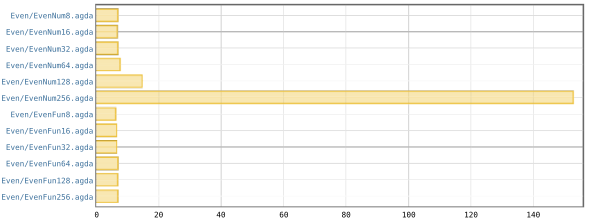
\includegraphics[scale=0.6]{benchmark-vanilla}
  \caption{Benchmark using original AutoInAgda}
  \label{fig:vanilla}
\end{figure}

\begin{figure}[h]
  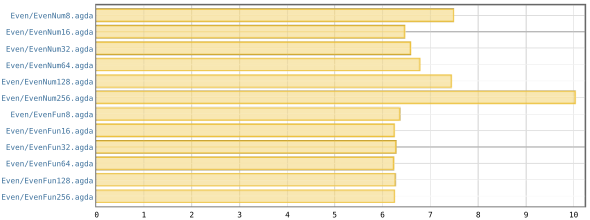
\includegraphics[scale=0.6]{benchmark}
  \caption{Benchmark using our implementation}
  \label{fig:our}
\end{figure}

As we can see from the results above, our implementation has made a big
improvement in terms of performance reaching for example in the case of
parameter 256 a improvement of $x15$. We were not able to benchmark the original
library in bigger inputs because the compile time would be too much.

For small cases the difference between implementations is
despicable, although is worthy to note that there is always a lower limit of
what we can achieve due to the requirement of Agda to check that every file we
depend on has been already typechecked.

\section{Conclusions and future work}
\label{sec:conclusions}

This work has explored the possibilities that the new Agda's metaprogramming API
has to offer in order to automatise program construction. We have been able as
shown in section \ref{sec:benchmark} to have a big performance boost with
regard to the original implementation of the AutoInAgda library in some cases
reaching a 15x boost.

However, we have also noted that expressive wise our library deeply depends on
how the internal |unify| (the one offered by the reflection API is just a
reflection of the one used internally by the typechecker) function should be
changed to allow automatic construction of more programs while retaining the
ones it is already able to solve.

We believe that intimate knowledge of the inner workings of Agda's inference and
typechecking algorithms is required to improve this situation. Nevertheless,
The situation is not that bad because we have designed our framework to be
|unify| agnostic. This is, we have parametrized the proof search by the
unification function so it can be easily interchanged and tested.

Moreover, we have introduced an implementation of some basic debugging
facilities that work both for the original AutoInAgda library and our extended
version, that should make the process of automatically filling Agda holes more
pleasant for the Agda's programmer or type theorist practitioner.

As a future line of work, we should be able to integrate our framework into a
sort of elaboration monad for metaprogramming as it was done by Christiansen and
Brady \cite{Christiansen:2016:ERE:2951913.2951932} in Idris. An attempt to
implement such elaboration monad can be found in the accompanying code of this
work under the folder \emph{ElaborationInAgda}.

\appendix

\bibliographystyle{plain}
\bibliography{bibliography}
\end{document}
